% L13a figure: the CRUD operations of a RESTful web service.
%
% A client sends four kinds of request to a lab's web service for its experiment
% records. Each lane shows the operation, the HTTP request, and what happens to
% the records: POST creates a new record, GET returns record 42 unchanged, PUT
% or PATCH updates record 42, and DELETE removes it. Blue marks the requests and
% what they change.
%
% Drawn on November 12, 2026 with the palette and build of the L12c figures.
% The notebook SVG carries a dark palette added by theme_svg.py; keep new colors
% in that script's mapping when changing the palette here.
\documentclass[tikz,border=4pt]{standalone}
\usepackage[no-math]{fontspec}
\IfFontExistsTF{Arial}{\setsansfont{Arial}}{\setsansfont{TeX Gyre Heros}}
\IfFontExistsTF{Menlo}{\setmonofont{Menlo}[Scale=0.88]}{}
\renewcommand{\familydefault}{\sfdefault}
\usepackage{amsmath,amssymb}
\usetikzlibrary{arrows.meta, calc, fit, backgrounds, positioning, decorations.pathreplacing}

% Ink, blue, gray, and band match the L12c figures.
\definecolor{vnink}{HTML}{202124}
\definecolor{gdblue}{HTML}{0091FF}
\definecolor{gdgray}{HTML}{6D7278}
\definecolor{waband}{HTML}{EEF0F2}
\definecolor{nodefill}{HTML}{FFFFFF}

\begin{document}
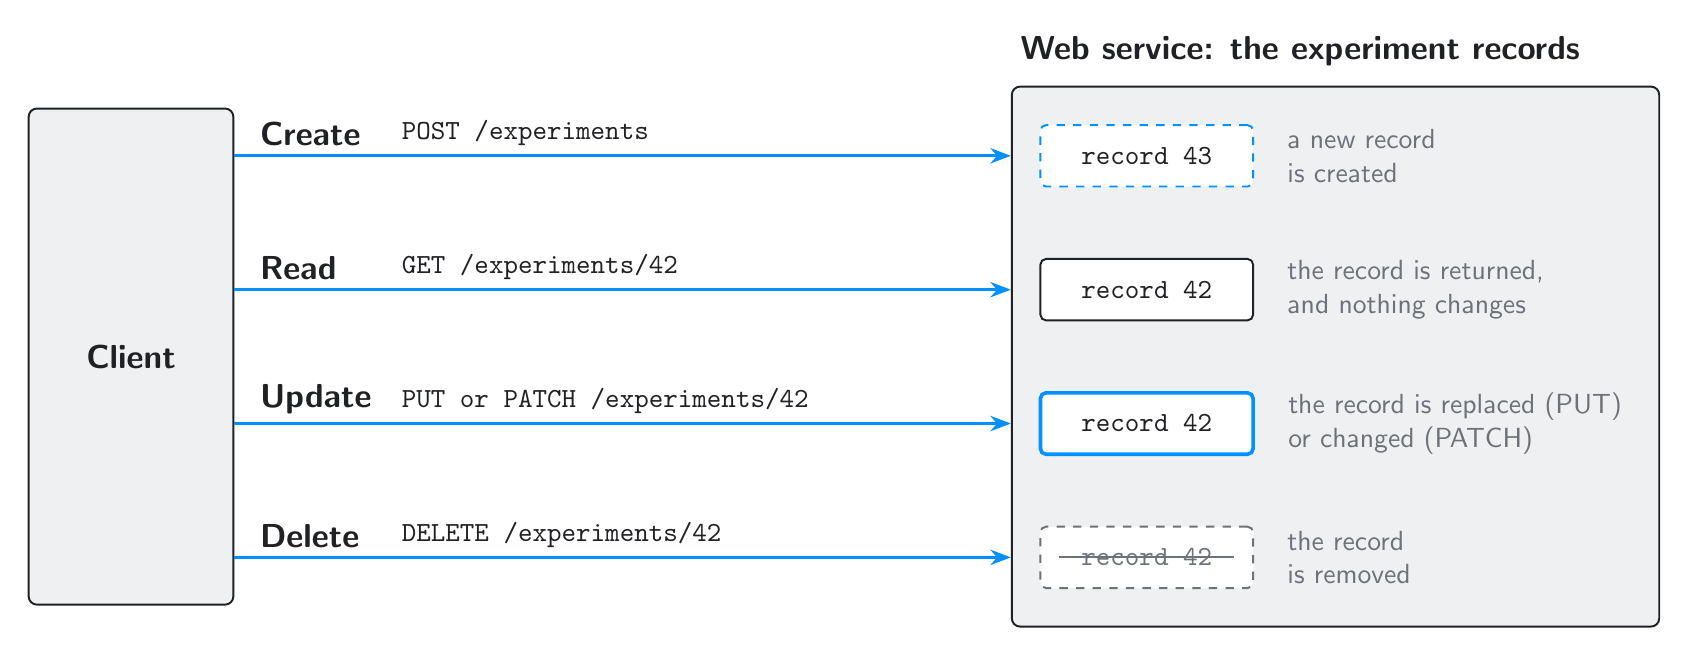
\begin{tikzpicture}[
  font=\sffamily\large,
  >={Stealth[length=2.6mm]},
  box/.style={draw=vnink, rounded corners=3pt, fill=waband, line width=0.7pt, text=vnink, align=center,
    font=\sffamily\large\bfseries},
  card/.style={draw=vnink, rounded corners=2pt, fill=nodefill, line width=0.7pt, font=\ttfamily\normalsize,
    text=vnink, minimum width=2.7cm, minimum height=0.78cm},
  op/.style={font=\sffamily\large\bfseries, text=vnink, anchor=south west, inner sep=2pt},
  req/.style={font=\ttfamily\normalsize, text=vnink, anchor=south west, inner sep=2pt},
  what/.style={font=\sffamily\normalsize, text=gdgray, anchor=west, align=left},
  request/.style={->, line width=1.0pt, draw=gdblue}
]

% ------------------------------------------------------------------ the client
\node[box, minimum width=2.6cm, minimum height=6.3cm] (client) at (0,-2.55) {Client};

% ------------------------------------------------------------------ the web service
\node[card, draw=gdblue, dashed] (c1) at (12.9, 0.00) {record 43};
\node[card]                      (c2) at (12.9,-1.70) {record 42};
\node[card, draw=gdblue, line width=1.3pt] (c3) at (12.9,-3.40) {record 42};
\node[card, draw=gdgray, dashed, text=gdgray] (c4) at (12.9,-5.10) {record 42};
\draw[draw=gdgray, line width=0.8pt] ($(c4.west)+(0.25,0)$) -- ($(c4.east)+(-0.25,0)$);

\node[what] (w1) at ($(c1.east)+(0.3,0)$) {a new record\\is created};
\node[what] (w2) at ($(c2.east)+(0.3,0)$) {the record is returned,\\and nothing changes};
\node[what] (w3) at ($(c3.east)+(0.3,0)$) {the record is replaced (PUT)\\or changed (PATCH)};
\node[what] (w4) at ($(c4.east)+(0.3,0)$) {the record\\is removed};

\begin{scope}[on background layer]
  \node[draw=vnink, rounded corners=3pt, fill=waband, line width=0.7pt, inner xsep=10pt, inner ysep=12pt,
    fit=(c1)(c4)(w1)(w2)(w3)(w4)] (service) {};
\end{scope}
\node[font=\sffamily\large\bfseries, text=vnink, anchor=south west] at ($(service.north west)+(0,0.12)$)
  {Web service: the experiment records};

% ------------------------------------------------------------------ the four requests
\foreach \card/\operation/\call in {
    c1/Create/{POST /experiments},
    c2/Read/{GET /experiments/42},
    c3/Update/{PUT or PATCH /experiments/42},
    c4/Delete/{DELETE /experiments/42}} {
  \draw[request] (client.east |- \card) -- (service.west |- \card);
  \node[op]  (o) at ($(client.east |- \card)+(0.25,0.05)$) {\operation};
  \node[req] at ($(client.east |- \card)+(2.05,0.05)$) {\call};
}

\end{tikzpicture}
\end{document}
